\subsection{Slučaj upotrebe: Kreiranje i dodeljivanje zadataka}

\subsubsection*{Kratak opis}

Projektni menadžer za izabrani film dodeljuje zadatke članovima produkcionog tima. Zadatak može da kreira i odmah dodeli (dodela novog zadatka) ili da dodeli zadatak koji već postoji, što uključuje i preraspodelu zadatka drugom članu (dodela postojećeg zadatka). Pri svakoj dodeli sistem proverava trenutne poslove izabranog člana, čuva dodelu i obaveštava člana o zadatku.

\subsubsection*{Akteri}
\begin{itemize}
    \item \textbf{Projektni menadžer} -- pokreće slučaj upotrebe. Želi da brzo raspodeli posao i da pri dodeli vidi ko je slobodan, a ko preopterećen.
    \item \textbf{Član produkcionog tima} -- prima obaveštenje o dodeljenom zadatku. Želi da na vreme sazna šta treba da uradi i do kada. To je opšti akter: u zavisnosti od vrste zadatka, to je Scenarista, Storyboarder, Dizajner, Animator, Audio dizajner ili Montažer.
\end{itemize}

\subsubsection*{Preduslovi}
\begin{itemize}
    \item Projektni menadžer je prijavljen na sistem.
    \item Film postoji u sistemu i za njega je formiran produkcioni tim.
\end{itemize}

\subsubsection*{Postuslovi}
\begin{itemize}
    \item Zadatak je sačuvan, u stanju ,,Dodeljen'' je i ima izvršioca.
    \item Izvršilac je obavešten o zadatku. Pri preraspodeli je obavešten i prethodni izvršilac.
    \item Pregled trenutnih poslova tima je ažuriran.
\end{itemize}

\subsubsection*{Osnovni tok}
\begin{enumerate}
    \item Projektni menadžer bira film i opciju za zadatke.
    \item Sistem prikazuje spisak zadataka filma, sa stanjem i izvršiocem svakog zadatka.
    \item Projektni menadžer bira jednu od opcija:
    \begin{enumerate}
        \item Ukoliko kreira nov zadatak, izvršava se podtok P1 (Dodela novog zadatka).
        \item Ukoliko dodeljuje zadatak koji već postoji, izvršava se podtok P2 (Dodela postojećeg zadatka).
    \end{enumerate}
    \item Sistem prikazuje članove produkcionog tima čija uloga odgovara vrsti zadatka, sa brojem trenutnih zadataka svakog člana.
    \item Projektni menadžer bira člana produkcionog tima i potvrđuje dodelu.
    \item Sistem proverava trenutne poslove izabranog člana.
    \item Sistem čuva dodelu i postavlja stanje zadatka na ,,Dodeljen''.
    \item Sistem istovremeno obaveštava izabranog člana o zadatku i ažurira pregled trenutnih poslova tima.
    \item Sistem prikazuje ažuriran spisak zadataka filma.
\end{enumerate}

Koraci 3--9 se ponavljaju dok projektni menadžer ima zadataka za dodelu.

\subsubsection*{Podtokovi}

\paragraph*{P1: Dodela novog zadatka}
\begin{enumerate}
    \item Sistem prikazuje formular za nov zadatak.
    \item Projektni menadžer unosi podatke o zadatku.
    \item Projektni menadžer potvrđuje unos.
    \item Sistem vrši validaciju podataka.
    \item Sistem čuva zadatak u stanju ,,Kreiran''. Proces se nastavlja u koraku 4 osnovnog toka.
\end{enumerate}

\paragraph*{P2: Dodela postojećeg zadatka}
\begin{enumerate}
    \item Projektni menadžer bira sa spiska zadatak u stanju ,,Kreiran'' ili ,,Dodeljen''.
    \item Sistem prikazuje podatke o zadatku i njegovog trenutnog izvršioca, ako ga ima. Proces se nastavlja u koraku 4 osnovnog toka.
\end{enumerate}

\subsubsection*{Alternativni tokovi}

\paragraph*{A1: Neuspešna validacija podataka}
\begin{itemize}
    \item U koraku 4 podtoka P1, ako sistem naiđe na neispravno popunjeno polje formulara, obeležava polje koje je potrebno ispraviti i obaveštava projektnog menadžera. Projektni menadžer ispravlja unos. Proces se nastavlja u koraku 3 podtoka P1.
\end{itemize}

\paragraph*{A2: Rok je posle roka faze}
\begin{itemize}
    \item U koraku 4 podtoka P1, ako je rok zadatka posle roka faze produkcije kojoj zadatak pripada, sistem prikazuje rok faze i traži izmenu. Projektni menadžer menja rok zadatka. Proces se nastavlja u koraku 3 podtoka P1.
\end{itemize}

\paragraph*{A3: Nema člana sa odgovarajućom ulogom}
\begin{itemize}
    \item U koraku 4 osnovnog toka, ako u produkcionom timu nema člana čija uloga odgovara vrsti zadatka, sistem o tome obaveštava projektnog menadžera. Zadatak ostaje u stanju u kom je bio. Proces se nastavlja u koraku 9 osnovnog toka.
\end{itemize}

\paragraph*{A4: Izabrani član je preopterećen}
\begin{itemize}
    \item U koraku 6 osnovnog toka, ako izabrani član ima više trenutnih zadataka od dozvoljenog, sistem prikazuje upozorenje.
    \item Ako projektni menadžer odluči da izabere drugog člana, proces se nastavlja u koraku 5 osnovnog toka.
    \item Ako projektni menadžer potvrdi dodelu, sistem beleži da je dodela potvrđena uprkos upozorenju. Proces se nastavlja u koraku 7 osnovnog toka.
\end{itemize}

\paragraph*{A5: Odustajanje od dodele}
\begin{itemize}
    \item U koraku 5 osnovnog toka, ako projektni menadžer odustane od dodele, zadatak ostaje u stanju u kom je bio: ,,Kreiran'', ili ,,Dodeljen'' sa dotadašnjim izvršiocem. Proces se nastavlja u koraku 9 osnovnog toka.
\end{itemize}

\paragraph*{A6: Preraspodela zadatka}
\begin{itemize}
    \item U koraku 8 osnovnog toka, ako je zadatak izabran u podtoku P2 već imao izvršioca, sistem obaveštava i prethodnog izvršioca da mu je zadatak oduzet. Proces se nastavlja u koraku 9 osnovnog toka.
\end{itemize}

\subsubsection*{Specijalni zahtevi}
\begin{itemize}
    \item Spisak članova tima sa brojem trenutnih zadataka prikazuje se za najviše dve sekunde.
\end{itemize}

\subsubsection*{Dodatne informacije}
\begin{itemize}
    \item Podaci o zadatku su: vrsta (scenario, storyboard, dizajn, animacija, zvuk, montaža), element produkcije na koji se odnosi (film, scena ili kadar), opis, rok i prioritet (nizak, srednji, visok).
    \item Vrsta zadatka određuje ulogu izvršioca: scenario -- Scenarista, storyboard -- Storyboarder, dizajn -- Dizajner, animacija -- Animator, zvuk -- Audio dizajner, montaža -- Montažer.
    \item Trenutni zadaci člana su zadaci u stanju ,,Dodeljen'' ili ,,Vraćen na doradu''. Član je preopterećen ako ima više od pet trenutnih zadataka.
    \item Obaveštenje sadrži naziv zadatka, film, rok i ime projektnog menadžera.
    \item Veze na dijagramu slučaja upotrebe: ,,Dodela novog zadatka'' i ,,Dodela postojećeg zadatka'' su dve vrste ovog slučaja (generalizacija) i opisane su podtokovima P1 i P2. ,,Provera trenutnih poslova člana'' (korak 6) i ,,Obaveštavanje člana produkcionog tima'' (korak 8) izvršavaju se uvek (\guillemotleft{}include\guillemotright{}). ,,Potvrda dodele preopterećenom članu'' izvršava se samo kada je izabrani član preopterećen (alternativni tok A4, \guillemotleft{}extend\guillemotright{}).
\end{itemize}


\begin{figure}[H]
	\centering
	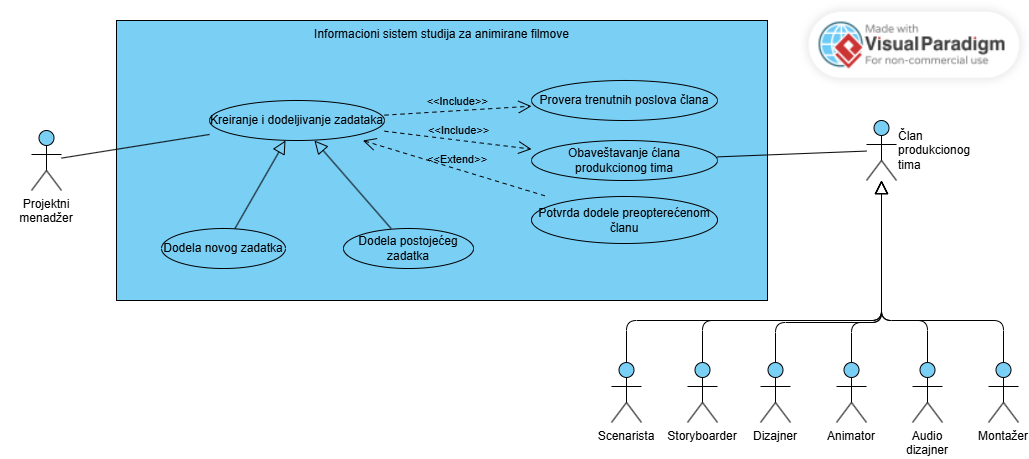
\includegraphics[width=\textwidth]{./dijagrami/dijagrami_slucajeva_upotrebe/kreiranje_i_dodeljivanje_zadataka.png}
	\caption{Dijagram slučaja upotrebe ,,Kreiranje i dodeljivanje zadataka''}
 \end{figure}

% \begin{figure}[H]
% 	\centering
% 	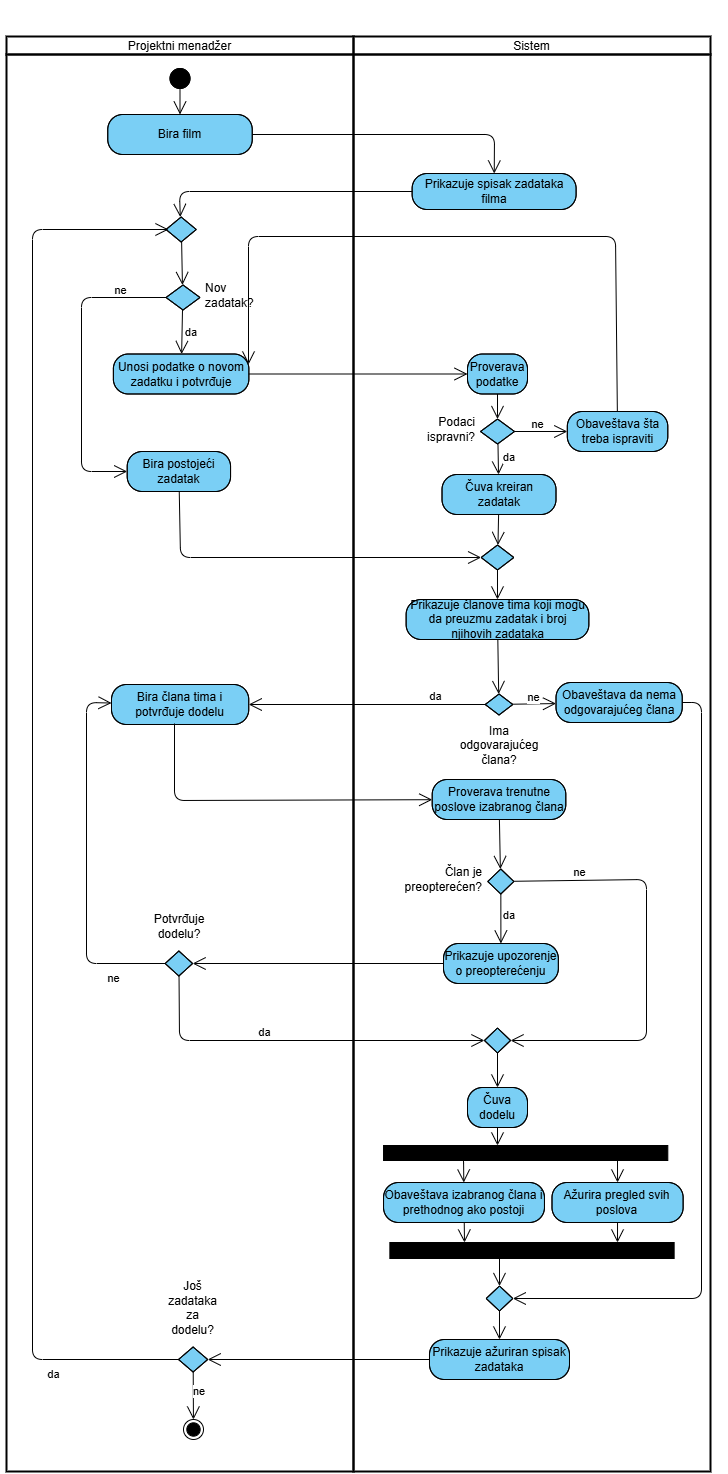
\includegraphics[width=\textwidth,height=0.85\textheight,keepaspectratio]{./dijagrami/dijagrami_aktivnosti/kreiranje_i_dodeljivanje_zadataka.png}
% 	\caption{Dijagram aktivnosti ,,Kreiranje i dodeljivanje zadataka''}
%  \end{figure}

% \begin{figure}[H]
% 	\centering
% 	\includegraphics[width=\textwidth]{./dijagrami/dijagrami_sekvence/kreiranje_i_dodeljivanje_zadataka.png}
% 	\caption{Dijagram sekvence ,,Kreiranje i dodeljivanje zadataka''}
%  \end{figure}

% \begin{figure}[H]
% 	\centering
% 	\includegraphics[width=\textwidth]{./dijagrami/dijagrami_stanja/zadatak.png}
% 	\caption{Dijagram stanja zadatka}
%  \end{figure}

\newpage
